% comment out for student version
\ifdefined\Student\relax\else\def\Teacher{}\fi

\documentclass[12pt]{article}

\title{Arithmetic Operators}
\author{Chris Mayfield and Helen Hu}
\date{Summer 2021}

%\ProvidesPackage{cspogil}

% fonts
\usepackage[utf8]{inputenc}
\usepackage[T1]{fontenc}
\usepackage{mathpazo}

% spacing
\usepackage[margin=2cm]{geometry}
\renewcommand{\arraystretch}{1.4}
\setlength{\parindent}{0pt}

% orphans and widows
\clubpenalty=10000
\widowpenalty=10000
\pagestyle{empty}

% figures and tables
\usepackage{graphicx}
\usepackage{multicol}
\usepackage{tabularx}
\usepackage{wrapfig}

% fixed-width columns
\usepackage{array}
\newcolumntype{L}[1]{>{\raggedright\let\newline\\\arraybackslash\hspace{0pt}}m{#1}}
\newcolumntype{C}[1]{>{\centering\let\newline\\\arraybackslash\hspace{0pt}}m{#1}}
\newcolumntype{R}[1]{>{\raggedleft\let\newline\\\arraybackslash\hspace{0pt}}m{#1}}

% include paths
\makeatletter
\def\input@path{{Models/}{../../Models/}}
\graphicspath{{Models/}{../../Models/}}
\makeatother

% colors
\usepackage[svgnames,table]{xcolor}
\definecolor{bgcolor}{HTML}{FAFAFA}
\definecolor{comment}{HTML}{007C00}
\definecolor{keyword}{HTML}{0000FF}
\definecolor{strings}{HTML}{B20000}

% table headers
\newcommand{\tr}{\bf\cellcolor{Yellow!10}}

% syntax highlighting
\usepackage{textcomp}
\usepackage{listings}
\lstset{
    basicstyle=\ttfamily\color{black},
    backgroundcolor=\color{bgcolor},
    numberstyle=\scriptsize\color{comment},
    commentstyle=\color{comment},
    keywordstyle=\color{keyword},
    stringstyle=\color{strings},
    columns=fullflexible,
    keepspaces=true,
    showlines=true,
    showstringspaces=false,
    upquote=true
}

% code environments
\newcommand{\java}[1]{\lstinline[language=java]{#1}}%[
\lstnewenvironment{javalst}{\lstset{language=java,backgroundcolor=}}{}
\lstnewenvironment{javabox}{\lstset{language=java,frame=single,numbers=left}\quote}{\endquote}

% PDF properties
\usepackage[pdftex]{hyperref}
\urlstyle{same}
\makeatletter
\hypersetup{
  pdftitle={\@title},
  pdfauthor={\@author},
  pdfsubject={\@date},
  pdfkeywords={},
  bookmarksopen=false,
  colorlinks=true,
  citecolor=black,
  filecolor=black,
  linkcolor=black,
  urlcolor=blue
}
\makeatother

% titles
\makeatletter
\renewcommand{\maketitle}{\begin{center}\LARGE\@title\end{center}}
\makeatother

% boxes [optional height]
\newcommand{\emptybox}[1][10em]{
\vspace{1em}
\begin{tabularx}{\linewidth}{|X|}
\hline\\[#1]\hline
\end{tabularx}}

% models
\newcommand{\model}[1]{\section{#1}\nopagebreak}
\renewcommand{\thesection}{Model~\arabic{section}}

% questions
\newcommand{\quest}[1]{\subsection*{Questions~ (#1)}}
\newcounter{question}
\newcommand{\Q}{\vspace{1em}\refstepcounter{question}\arabic{question}.~ }
\renewcommand{\thequestion}{\#\arabic{question}}

% sub-question lists
\usepackage{enumitem}
\setenumerate[1]{label=\alph*)}
\setlist{itemsep=1em,after=\vspace{1ex}}

% inline answers
\definecolor{answers}{HTML}{C0C0C0}
\newcommand{\ans}[1]{%
\ifdefined\Student
    \leavevmode\phantom{~~\textcolor{answers}{#1}}
\else
    ~~\textcolor{answers}{#1}
\fi}

% longer answers [optional height]
\newsavebox{\ansbox}
\newenvironment{answer}[1][4em]{
\nopagebreak
\begin{lrbox}{\ansbox}
\begin{minipage}[t][#1]{\linewidth}
\color{answers}
}{
\end{minipage}
\end{lrbox}
\ifdefined\Student
    \phantom{\usebox{\ansbox}}%
\else
    \usebox{\ansbox}%
\fi}


\begin{document}

\maketitle

Now that you've written a few programs, let's take a step back and discuss how to do basic arithmetic.
The behavior of Java operators (+, -, *, /, \%) depends on the type of data you have.

\rolenames

\guide{
  \item Summarize the benefits of working as a team.
  \item Evaluate Java expressions that use the \% operator with integers.
  \item Explain the difference between integer and floating-point division.
  \item Identify operator precedence for addition, division, and assignment.
}{
  \item Recognizing mathematical operations based on tables. (Information Processing)
}{
This activity focuses on integer vs floating-point division and operator precedence.
Students should understand how to declare and assign variables before completing this activity.
The meta activity at the beginning reinforces the idea of working together as a team.

\ref{mints} refers to the instructor hypothetically giving mints to teams to divide among themselves.
Consider bringing real mints to build rapport with the class.
You can use other small objects like paperclips.
When reporting out, introduce the terms \emph{remainder operator}, \emph{modulo operation}, and \emph{modulus}.
Explain that ``x \% y'' is pronounced ``x mod y''.

On \ref{dividing-numbers.tex}, you may need to point out (after students work for a while) that it makes no difference whether a floating-point number ends with a zero.
In other words, \java{4.} is the same value as \java{4.0}.
%
For \ref{intdiv}, have at least 2--3 teams share their answers with the class to encourage different ways of thinking about the concepts (and how to put them into words).

On \ref{order-operations.tex}, help students understand that assignment is an operation (in contrast to the equals sign in mathematics).
At the end of the activity, invite teams to discuss what the \emph{assignment operation} is in terms of what computer hardware does.

Key questions: \ref{modoper}, \ref{intdiv}, \ref{key3}
}

% Based on Model 1 of "We Are a Learning Team!" by Urik Halliday

\model{Group vs Team}

Throughout the course, you will need to examine and process information, ask and answer questions, construct your own understanding, and develop new problem-solving skills.

\begin{center}
% source: http://www.clipartpanda.com/categories/group-prayer-images

\includegraphics[height=2.25in]{group1.png}
\hspace{0.5in}
% source: http://www.clipartpanda.com/categories/working-together-as-a-team

\includegraphics[height=2.25in]{group2.jpg}
\end{center}


\quest{8 min}


\Q What are some advantages to working in groups/teams?

\begin{answer}[5em]
You get to know other people and make new friends.
Different people have different backgrounds and skills.
The responsibility is shared.
\end{answer}


\Q What are some disadvantages to working in groups/teams?

\begin{answer}[5em]
Some group members may decide not to contribute.
One or two students may be absent.
People may not always get along with each other.
\end{answer}


\Q What is the difference between a group and a team?
Come up with a precise answer.

\begin{answer}[5em]
A group is students who just sit by each other and turn in the same assignment.
A team actually works together toward a common goal, drawing on each other's strengths.
\end{answer}


\Q How can working as a team help you accomplish the tasks described in \ref{group-vs-team.tex}?
Give at least two specific examples.

\begin{answer}[5em]
Working as a team makes it easier to examine and process information, because different people have different perspectives.
We can also develop new problem-solving skills by observing how each other approaches the problems.
\end{answer}

\model{The \% Operator}
% Based on Model 2 of "Activity 01 - Operators" by Helen Hu

\vspace{-1ex}
\begin{center}
\begin{tabular}[t]{|C{35pt}|C{65pt}|C{35pt}|}
\hline
 9 / 4 & \textit{evaluates to} & 2 \\
\hline
10 / 4 & \textit{evaluates to} & 2 \\
\hline
11 / 4 & \textit{evaluates to} & 2 \\
\hline
12 / 4 & \textit{evaluates to} & 3 \\
\hline
13 / 4 & \textit{evaluates to} & 3 \\
\hline
14 / 4 & \textit{evaluates to} & 3 \\
\hline
15 / 4 & \textit{evaluates to} & 3 \\
\hline
16 / 4 & \textit{evaluates to} & 4 \\
\hline
\end{tabular}
\hspace{0.5in}
\begin{tabular}[t]{|C{35pt}|C{65pt}|C{35pt}|}
\hline
 9 \% 4 & \textit{evaluates to} & 1 \\
\hline
10 \% 4 & \textit{evaluates to} & 2 \\
\hline
11 \% 4 & \textit{evaluates to} & 3 \\
\hline
12 \% 4 & \textit{evaluates to} & 0 \\
\hline
13 \% 4 & \textit{evaluates to} & 1 \\
\hline
14 \% 4 & \textit{evaluates to} & 2 \\
\hline
15 \% 4 & \textit{evaluates to} & 3 \\
\hline
16 \% 4 & \textit{evaluates to} & 0 \\
\hline
\end{tabular}
\end{center}


\quest{12 min}


\Q Which numbers \% 4 evaluate to 0 in the table above?
If the table were extended to include more rows, which other numbers \% 4 would evaluate to 0?

\begin{answer}
12 and 16. Other numbers include 0, 4, 8, 20, 24.
\end{answer}


\Q Look at the expressions in the second table that evaluate to 1.
How do the left operands in these expressions (9, 13, 17) differ from those that evaluate to 0?

\begin{answer}
They differ by one.
\end{answer}


\Q List three numbers \% 5 that will evaluate to 0 and three numbers \% 5 that will evaluate to 2.

\begin{answer}
0, 5, 10 and 2, 7, 12.
\end{answer}


\Q Evaluate the following Java expressions:

\begin{center}
\begin{tabular}{C{1in}C{1in}C{1in}C{1in}}
18 \% 4 \ans[3em]{= ~2} &
19 \% 4 \ans[3em]{= ~3} &
19 \% 5 \ans[3em]{= ~4} &
19 \% 6 \ans[3em]{= ~1} \\
\end{tabular}
\end{center}


\newpage

\Q Consider how you were taught to do long division in elementary school.
Finish solving for $79 \div 5$.
What is the answer?

\begin{center}
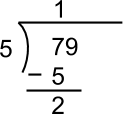
\includegraphics[scale=0.65]{div79by5.png}
\end{center}

\begin{answer}[3em]
We first bring the 9 down, then 5 goes into 29 five times, and so we subtract 25. The final answer is 15 remainder 4.
\end{answer}


\Q \label{mints}
Imagine that you are given candy mints to divide evenly among your team members.

\begin{enumerate}
\item If your team receives 11 mints, how many mints are left over?

\ans{\java{11 \% 4} is 3 ~~or~~ \java{11 \% 5} is 1}

\item If your team receives 2 mints, how many mints are left over?

\ans{\java{2 \% 4} is 2 ~~or~~ \java{2 \% 5} is 2}
\end{enumerate}


\Q \label{modoper}
Describe what the \% operator does.
How are the / and \% operators related?

\begin{answer}
Both operators divide two numbers: \% returns the remainder, and / returns the quotient.
\end{answer}


\Q \label{modreal}
Would it make sense to apply the \% operator to real numbers?
Why or why not?

\begin{answer}
Not really, since the concept of remainder is based on integer division.

(BTW floating-point modulo is defined in IEEE 754, but its use is rare.)
\end{answer}

\newpage
% Based on Models 3 and 4 of "Activity 01 Operators" by Helen Hu

\model{Dividing Numbers}
\label{CS1/oper-precedence}

\vspace{-1em}
\begin{center}
\renewcommand{\arraystretch}{1.4}
\begin{tabular}[t]{|C{35pt}|C{65pt}|C{35pt}|}
\hline
 9 / 4 & \textit{evaluates to} & 2 \\
\hline
10 / 4 & \textit{evaluates to} & 2 \\
\hline
11 / 4 & \textit{evaluates to} & 2 \\
\hline
12 / 4 & \textit{evaluates to} & 3 \\
\hline
13 / 4 & \textit{evaluates to} & 3 \\
\hline
14 / 4 & \textit{evaluates to} & 3 \\
\hline
15 / 4 & \textit{evaluates to} & 3 \\
\hline
16 / 4 & \textit{evaluates to} & 4 \\
\hline
\end{tabular}
\hspace{0.5in}
\begin{tabular}[t]{|C{45pt}|C{65pt}|C{45pt}|}
\hline
9    / 4.0 & \textit{evaluates to} & 2.25 \\
\hline
10   / 4.  & \textit{evaluates to} & 2.5 \\
\hline
11.  / 4   & \textit{evaluates to} & 2.75 \\
\hline
12   / 4.0 & \textit{evaluates to} & 3.0 \\
\hline
13   / 4.  & \textit{evaluates to} & 3.25 \\
\hline
14.0 / 4   & \textit{evaluates to} & 3.5 \\
\hline
15   / 4.0 & \textit{evaluates to} & 3.75 \\
\hline
16   / 4.  & \textit{evaluates to} & 4.0 \\
\hline
\end{tabular}
\end{center}


\quest{15 min}

\Q In the first table, which number(s) divided by 4 evaluate to 3?
What is significant about the number of answers you have written down?

\begin{answer}
12, 13, 14, and 15.
There are four answers, and we divided by four.
\end{answer}


\Q How do the answers in the first table differ from the second table?

\begin{answer}
The second table is mathematically correct; the first table rounds down.
\end{answer}


\Q To the right of the second table, round each answer to the closest integer.
How do those values compare to what you see in the first table?

\begin{answer}
The pattern is off by two rows.
The 0.5 and 0.75 values round up, but in the first table they don't.
\end{answer}


\Q Carefully explain the difference between the numbers in the first and second tables.

\begin{answer}
All the numbers in the first table have no decimal points.
At least one number in each row of the second table as a decimal point.
\end{answer}


\Q Complete the table:
\hspace{2em}
\begin{minipage}{0.5\textwidth}
\renewcommand{\arraystretch}{1.4}
\begin{tabular}[t]{|C{45pt}|C{65pt}|C{45pt}|}
\hline
14. / 4. & \textit{evaluates to} & \ans{3.5} \\
\hline
14. / 4  & \textit{evaluates to} & \ans{3.5} \\
\hline
14  / 4. & \textit{evaluates to} & \ans{3.5} \\
\hline
14  / 4  & \textit{evaluates to} & \ans{3}   \\
\hline
\end{tabular}
\end{minipage}


\Q Dividing numbers with fractional parts (known as \textbf{floating-point} numbers) gives you different results from dividing two integers.
In the previous question:

\begin{enumerate}
\item Which rows evaluate to an integer? \ans{the first three}
\vspace{1ex}
\item Which rows evaluate to a floating-point number? \ans{the last one}
\vspace{1ex}
\end{enumerate}


\Q Imagine you are writing a Java program that requires division.

\begin{enumerate}
\item What must be true about the \textbf{operands} (the numbers around the \textbf{operators}) for you to get the mathematically correct answer?

\ans{At least one of them needs to be a floating-point number.}
\vspace{1ex}

\item Does it need to be true for both operands? \ans{No}
\vspace{1ex}
\end{enumerate}


\Q Consider what you know about addition (\java{+}).
If you add two integers in a Java expression, will the result always be mathematically correct?
Justify your answer.

\begin{answer}
Yes, because adding two integers always results in an integer.
(Unless the number gets too large and the arithmetic overflows.)
\end{answer}


\Q What about subtraction (\java{-}) and multiplication (\java{*})? If you subtract or multiply two integers, will the answer always be mathematically correct? Justify your answer.

\begin{answer}
Yes, because subtraction and multiplication can be rewritten in terms of addition.
Division is the only special case, because it has both a quotient and a remainder.
\end{answer}

\model{Order of Operations}
% Based on Model 2 of "Activity 02 Declaration" by Helen Hu

Java follows a specific order for math and other operations. For example, multiplication and division take \emph{precedence} over addition and subtraction.
The following table lists several Java operators from highest precedence to lowest precedence.

\begin{center}
\begin{tabular}{|L{3in}|L{1in}|}
\hline
Parenthesis
& \tt ( ) \\
\hline
Unary (positive or negative signs)
& \tt + - \\
\hline
Multiplicative
& \tt * / \% \\
\hline
Additive
& \tt + - \\
\hline
Assignment
& \tt = \\
\hline
\end{tabular}
\end{center}

For the following questions, assume you have these two variables:

\begin{javalst}
    int x;
    double y;
\end{javalst}


\quest{10 min}


\Q What operator has the lowest precedence?
Why do you think Java is designed that way?

\begin{answer}
Assignment has the lowest precedence so that all other operations happen first (before the final value is stored in memory).
\end{answer}


\Q What operator has the highest precedence?
Why do you think Java is designed that way?

\begin{answer}
Parenthesis have the highest precedence so that you can impose a specific order.
For example, \java{2 * (3 + 4)} will perform addition before multiplication.
\end{answer}


\Q The \java{+} and \java{-} operators show up twice in the table of operator precedence.
For the Java statement ~\java{x = 5 * -3;} explain how you know whether the \java{-} operator is being used as an \emph{unary} or \emph{binary} operator.

\begin{answer}
It matters what is to the left or right of the operator.
In this example, the \java{-} is preceded by a \java{*}, so it must be unary.
\end{answer}


\newpage

\Q Determine the order of operations in the statement: ~ \java{x = 5 * -3;}

\begin{enumerate}[itemsep=2pt]
\item First operator to be evaluated: \ans[3em]{\java{-}}
\item Second operator: \ans[3em]{\java{*}}
\item Third operator: \ans[3em]{\java{=}}
\end{enumerate}


\Q Determine the order of operations in the statement: ~ \java{y = 9 / 2;}

\begin{enumerate}[itemsep=2pt]
\item First operator to be evaluated: \ans[3em]{\java{/}}
\item Second operator: \ans[3em]{\java{=}}
\end{enumerate}


\Q \label{key3}
Based on your answer to the previous question, explain why the variable \java{y} would be assigned 4.0 (as opposed to 4 or 4.5).

\begin{answer}
Since \java{y} is a floating-point variable, the integer result 4 would be stored as 4.0 in memory.
\end{answer}


\Q Rewrite the assignment for \java{y} so that it would be set correctly to 4.5. (Hint: you'll need to recall what you learned about division in \ref{dividing-numbers.tex}.)

\begin{answer}
\java{y = 9.0 / 2.0;}
\end{answer}


\end{document}
